\documentclass[parskip=full]{scrartcl}
\usepackage[utf8]{inputenc} % use utf8 file encoding for TeX sources
\usepackage[T1]{fontenc}    % avoid garbled Unicode text in pdf
\usepackage[german]{babel}  % german hyphenation, quotes, etc
\usepackage{hyperref}       % detailed hyperlink/pdf configuration
\usepackage{graphicx}       % provides commands for including figures
\usepackage{csquotes}       % provides \enquote{} macro for "quotes"
\usepackage[nonumberlist]{glossaries}     % provides glossary commands
\usepackage{enumitem}
\usepackage{setspace}
\usepackage{subfigure}
\usepackage{pgf}

\makenoidxglossaries

\newglossaryentry{nn}
{
	name={neural network},
	description={a network or a circuit of neuron used for information processing inspired by the way biological neural systems process data},
	plural=neural networks
}

\newglossaryentry{img}
{
	name={image},
	description={a two dimensional matrix of red,green,blue (RGB) values that can be visualized as each cell represents a single pixel on the monitor. (ex.: a photo)},
	plural=images
}

\newglossaryentry{cpu}
{
	name={CPU},
	description={Central Processing Unit},
	plural=CPUs
}

\newglossaryentry{fpga}
{
	name={FPGA},
	description={Field Programmable Gate Array},
	plural=FPGAs
}

\newglossaryentry{gpu}
{
	name={GPU},
	description={A graphics processing unit. It is a specialized electronic circuit designed to rapidly manipulate and alter memory to accelerate the creation of images in a frame buffer intended for output to a display device.},
	plural=GPUs
}

\newglossaryentry{json}
{
	name={JSON},
	description={JavaScript Object Notation},
}

\newglossaryentry{xml}
{
	name={XML},
	description={Extensible Markup Language},
}

\newglossaryentry{dp}
{
	name={deployment platform},
	plural={deployment platforms},
	description={Hardware to run the calculations on. (ex.: FPGA or CPU)},
}

\newglossaryentry{image classification}
{
	name={image classification},
	description={Detection of what object is shown in a given picture, that is then matched to a fitting class.},
}

\newglossaryentry{power consumption}
{
	name={power consumption},
	description={idek},
}

\newglossaryentry{host pc}
{
	name={host pc},
	description={The main computer that is interacted with and used for input and output. },
}

\newglossaryentry{bb}
{
	name={bounding box},
	plural={bounding boxes},
	description={Rectangle indicating the outer edges of an object in an image.},
}

\newglossaryentry{performance}
{
	name={performance},
	description={idek},
}

\newglossaryentry{ic}
{
	name={image class},
	plural={image classes},
	description={idek},
}

\title{Specifications}
\author{}
\begin{document}
\renewcommand{\figurename}{Figure}
\begin{titlepage}
\centering
	\vspace{3cm}
	{\scshape\LARGE Praxis der Softwarentwicklung\par}
	\vspace{2cm}
	{\scshape\Huge\bfseries Specificationsbook \par}	
	\vspace{2cm}
	{\scshape\Huge\bfseries Neural Network based Image Classification System on Heterogeneous Platforms \\ Team 2 \par}
	\vspace{2cm}
	{\Large from \par}
	\vspace{0.25cm}
	{\Large Dimitrov, Drehwald, Guneshka, Häring, Stangel \par}
	\vfill
\end{titlepage}
\newpage
\tableofcontents
\newpage
\section{Introduction}
In todays world of globalisation and digitalisation, to keep up with the rapidly growing economy, one important challenge is the automatisation of tasks. One aspect of this is the classification of visual inputs. Whether it is to check for broken parts in production or surveillance of public places. With the rapidly growing power of computers, neural networks are becoming more popular for tasks like this, as they need a lot of computational power but deliver sufficiently accurate results.\\
In the following project we want to build a framework with an intuitive graphical user interface to achieve these kinds of tasks.\\
To speed up the process of classification the software will be able to use different hardware that is more efficient for specific calculations. To further adjust the neural network to its task it should have different modes to function on. High \gls{performance}, low \gls{power consumption} and a high energy effiency mode. \\


\section{Goal}
The goal of this project is to create a software which performs sufficiently accurate \gls{image classification} and is able to switch between \glspl{dp} and working modes. The software will be able to predict the \gls{power consumption} and the performance (bandwidth, FLOPs).\\
The software should also have a GUI to interact with the program and to visualise the results.\\
The software should be extendable for further tasks.


\section{Product use}
The target group are engineers with a basic knowledge of data science.\\
The software is used to classify images on different deployment platforms with different working modes using a pretrained neural network.\\
Additionally, the software can be extended to be used for image detection, classification of frames from a videostream and training of a \gls{nn}.\\


\section{Criteria}
\subsection{Must Acceptance criteria}
\begin{tabular}{p{2cm}p{12cm}}
<<<<<<< HEAD
\textbf{MAC010} & \textbf{Image classification} \\
& The software can take a single image as input and returns the possiblities for each predefined \gls{ic}. The prediction is based on a pretrained neural network.\\
\textbf{MAC020} & \textbf{Running \gls{nn} on heterogeneous platforms} \\
& The software is able to communicate with \gls{cpu} and \gls{fpga}. The software is able to offload calculations to the different \glspl{dp} and receive the results.\\
\textbf{MAC030} & \textbf{Different operating modes} \\
& The software has three modes. One mode for high perfomance, one for low \gls{power consumption} and one for high energy efficiency. \\
\textbf{MAC040} & \textbf{Performance and \gls{power consumption} prediction}\\
& The software can predict the \gls{performance} with a certain \gls{power consumption} and also the \gls{power consumption} for a certain \gls{performance}.\\
\textbf{MAC050} & \textbf{GUI for interacting with software} \\
& The user is able to access the entire functionality described in MAC10-MAC40 just by using the GUI. No coding or command line usage is required.
\end{tabular}

\subsection{Can Acceptance criteria}
\begin{tabular}{p{2cm}p{12cm}}
\textbf{CAC070} & \textbf{Illustration of the topology of a \gls{nn}} \\
& The software is able to visualize the topology of a given \gls{nn}(see figure 7). \\
\textbf{CAC071} & \textbf{The visualized nn can be saved}\\
& The visualized \gls{nn} is saved as a .png file in a chosen directory.\\
\textbf{CAC080} & \textbf{Object Detection} \\
& The software can detect the \gls{bb} of an object. \\ 
\textbf{CAC090} &  \textbf{Using different models}\\
& The user is able to use different pretrained \glspl{nn} before an \gls{image classification} process. \\
\textbf{CAC100} & \textbf{Training \glspl{nn}} \\
& The software allows the user to train a \gls{nn} based on an predefined architecture.\\
& Neural networks trained by the user will be executed the same way neural networks provided with the software are executed.\\
\textbf{CAC110} & \textbf{Voting of multiple \glspl{nn}} \\
& The user is able to choose multiple \glspl{nn} for classification.\\
& The software will then execute all selected neural networks sequentially. The result presented to the user will be based on the weighted results of the different \glspl{nn}.\\
\textbf{CAC120} & \textbf{Using video for classification} \\
& The software is able to take a video, divide it into a certain amount of frames and perform \gls{image classification} for each frame.\\
& The classified frames are shown and can be iterated by the user. \\
\textbf{CAC130} & \textbf{Using camera for classification as input} \\
& The software takes the current frame from the camera connected to the \gls{host pc}, classifies it, displays the results and then when ready, takes the next available frame.\\
\textbf{CAC140} & \textbf{Running \gls{nn} on \gls{gpu}}\\
& MAC20 is extended by \gls{gpu}.\\
\end{tabular}

\subsection{Criteria of demarcation}
\begin{tabular}{p{2cm}p{12cm}}
\textbf{D010} & \textbf{No low-level optimization}\\
& Optimisations to reduce the execution time of object classification and detection will  be carried out in OpenCL.\\
& No optimizations including low-level languages or assembly intrinsics will be implemented.\\
&\\
\textbf{D020} & \textbf{No real time requirements}\\
& The software doesn't have to react in realtime. \\
& Code optimizations will be done in OpenCL to reduce the running time of the network per \gls{image classification}/ detection task.\\
&\\
\textbf{D030} & \textbf{No neural network size optimization}\\
& No techniques for memory usage reduction like parameter sharing, prunning or binarization will be implemented.\\
&\\
\textbf{D040} & \textbf{No mobile support}\\
& The software does not support mobile devices, like smartphones or wearables.\\
& \\
\textbf{D050} & \textbf{No input from commandline}\\
& The software does not support commandline input. The features are only useable with the GUI.
\end{tabular}


\section{Product environment}
The software runs on a computer in the lab at the CDNC institute. It has a CPU and an external FPGA connected via USB. Additionally, there is a \gls{gpu}.\\ 
The operating system is XUbuntu 18.04.


\section{Productdata}
\begin{tabular}{p{2cm}p{11.4cm}}
\textbf{PD010} & \textbf{Images for classification}\\
& The user can choose images of the format .jpg, .png, .bmp. The images are chosen by the user with the file explorer.\\
\textbf{PD020} & \textbf{Config/weight file of pretrained model}\\
& The config file is a .cfg file.\\
& In the beginning the classes and output nodes are mapped. In the format \textit{<id of output node> = <classname>}\\
& Then the hyperparameters are described with the format \textit{<name> = <value>}. Then the layers are described in their order with the following format\\
& \textit{\lbrack kind of layer\rbrack}\\
& list of parameters in the format \textit{<name> = <value>}\\
& Then the weights and biases for each layer are listed.\\
\textbf{PD030} & \textbf{Labeled image set for classification training}\\
& The dataset is chosen by the user. The dataset is a directory with images and the image name has the format \textit{<id of image>\_<image class>}.\\
\textbf{PD040} & \textbf{Labeled set of images for object detection training}\\
& It is a .txt file in the same directory as the images. The images are labeled with their name. The \gls{bb} for each image are described in the .txt file with the same name as the image, in the format \textit{\gls{ic}, x, y, width, height}. (X,Y) are the coordinates of the left bottom corner. (X, Y), width and height are relative values. 
\end{tabular}


\section{Functional Requirements Must}
\begin{tabular}{p{2cm}p{12cm}}
\textbf{MFR010} & \textbf{Use \gls{nn} for \gls{img} classification}\\                                     
& A \gls{nn} is used to classify \glspl{img}. The result is a list of probabilities for each \gls{ic}.\\
\textbf{MFR011} & \textbf{Deploy a pre-trained \gls{nn} with the corresponding layers}\\
& A pre-trained \gls{nn} is deployed with its layers to a specified platform. The deployed \gls{nn} is used for MFR010.\\
\textbf{MFR012} & \textbf{Reading and parsing a \gls{nn} configuration/weight file}\\
& The software is able to read a configuration file of a \gls{nn} and parse it for MFR011.\\
& \\
\textbf{MFR013} & \textbf{Implementation of layers}\\
& A \gls{nn} uses different layers with different properties. Convolutional, normalisation, dropout, fully connected, max pooling, softmax, depth concation layers have to be implemented. \\
& \\
\textbf{MFR020} & \textbf{High \gls{performance} operating mode}\\                                     
& An operating mode to perform calculations as fast as possible.\\
\textbf{MFR021} & \textbf{Low \gls{power consumption} operating mode}\\                                     
& An operating mode to perform calculations with low \gls{power consumption}.\\
\textbf{MFR022} & \textbf{Have high energy efficiency operating mode}\\                                     
& An operating mode to perform calculations at an optimal ratio between \gls{performance} and \gls{power consumption}.\\
\textbf{MFR023} & \textbf{Calculator for \gls{power consumption}}\\                                     
& The software can calculate the \gls{power consumption} of a given \gls{nn}, operating mode and \gls{dp}.\\
\textbf{MFR024} & \textbf{Calculator for \gls{performance}}\\                                     
& The software can calculate the \gls{performance} of a given \gls{nn}, operating mode and \gls{dp}.\\
\end{tabular}


\section{Productdata}
\begin{tabular}{p{2cm}p{11.4cm}}
\textbf{PD010} & \textbf{Images for classification}\\
& The user can choose images of the format .jpg, .png, .bmp. The images are chosen by the user with the file explorer.\\
& \\
\textbf{PD020} & \textbf{Config/weight file of pretrained model}\\
& The config file is a .cfg file.\\
& In the beginning the classes and output nodes are mapped. In the format \textit{number of output node = classname}\\
& Then the hyperparameters are described with the format \textit{<name> = <value>}. Then the layers are described in their order with the following format\\
& \textit{\lbrack kind of layer\rbrack}\\
& list of parameters in the format \textit{<name> = <value>}\\
& Then the weights and biases for each layer are listed.\\
& \\
\textbf{PD030} & \textbf{Labeled image set for classification training}\\
& The dataset is chosen by the user. The dataset is a directory with images and the image name has the format \textit{<id of image>\_<image class>}.\\
& \\
\textbf{PD040} & \textbf{Labeled set of images for object detection training}\\
& It is a .txt file in the same directory as the images. The images are labeled with their name. The bounding box for each image are described in the .txt file with the same name as the image, in the format \textit{image class, x, y, width, height}. (X,Y) are the coordinates of the left bottom corner. (X, Y), width and height are relative. \\
& \\
\textbf{PD050} & Output format of image classification results if saved\\
& If the output result of the classification is saved this is saved as a .txt file with the name of the image. The format is \textit{<image class name> = <prohability>}, one row for each image class.\\
& If multiple images are classified, there are multiple .txt files.\\
& \\
\textbf{PD060} & Output format of image detection results if saved\\
& If the output result of the detection is saved this is saved as a .txt file with the name of the image. The format is \textit{<image class name> = <prohability>, <X>, <Y>, <width>, <height>}, one row for each image class.\\
& If multiple images are detected, there are multiple .txt files.\\
& \\
\textbf{PD070} & \textbf{Video input}\\
& The input video is a .avi format.
\end{tabular}


\section{Functional Requirements Must}
\begin{tabular}{p{2cm}p{12cm}}
\textbf{MFR010} & \textbf{Use \gls{nn} for \gls{img} classification}\\                                     
& A \gls{nn} is used to classify \glspl{img}. The result is a list of prohabilities per image class.\\
\textbf{MFR011} & \textbf{Deploy pre-trained \gls{nn} with the corresponding layers}\\
& A pre-trained \gls{nn} is deployed with its layers to a specified platform. The deployed \gls{nn} is used for MFR010.\\
\textbf{MFR012} & \textbf{Reading and parsing a \gls{nn} configuration/weight file}\\
& The software is able to read a configuration file of a \gls{nn} and parse it for MFR011.\\
& \\
\textbf{MFR020} & \textbf{High performance operating mode}\\                                     
& An operating mode to perform calculations as fast as possible.\\
\textbf{MFR021} & \textbf{Low power consumption operating mode}\\                                     
& An operating mode to perform calculations with low power consumption.\\
\textbf{MFR022} & \textbf{Have high energy efficiency operating mode}\\                                     
& An operating mode to perform calculations at an optimal ratio between performance and power consumption.\\
\textbf{MFR023} & \textbf{Calculator for power consumption}\\                                     
& The software can calculate the power consumption on a given \gls{nn}, operating mode and deployment platform.\\
\textbf{MFR024} & \textbf{Calculator for performance}\\                                     
& The software can calculate the performance on a given \gls{nn}, operating mode and deployment platform.\\
\textbf {MFR025} & \textbf{Dispatching the calculation process defined from the mode}\\
& Tested with: Implements: \\
& The software is able to control the clock rate of the processor according to chosen operating mode. \\
& \\
\textbf {MFR030} & \textbf{Support CPU for calculation} \\
& Tested with: Implements \\
& The software supports CPU for calculation. \\
& \\
\end{tabular}
\newpage
\begin{tabular}{p{2cm}p{12cm}}
\textbf {MFR031} & \textbf{Support FPGA for calculation} \\
& Tested with: Implements: \\
& The software supports FPGA for calculation. \\
& \\
\textbf {MFR040} & \textbf{Send image for classification} \\
& Tested with: Implements: \\
& The software gives the image as input for the \gls{nn} to the chosen \gls{dp}. \\
& \\
\textbf {MFR041} & \textbf{Receive result} \\
& Tested with: Implements \\
& The program should be able to receive results of the executed \gls{image classification} from the \glspl{dp}. \\
& The software gives the image as input for the {nn} to the chosen deployment platform. \\
& \\
\textbf {MFR050} & \textbf{GUI} \\
& Tested with: Implements: \\
& The program has a Graphical User Interface to display all functions to the user. \\
& \\
\textbf {MFR060} & \textbf{Showing results} \\
& Tested with: Implements\\
& After executing the \gls{image classification}, the results are shown in a bar chart. \\
& \\
\textbf{MFR070} & \textbf{Choosing image for classification}\\
& Testet with: Implements: \\
& The GUI has a button with an on click event which opens a file explorer. The explorer filters the files that only files of the format .jpg, .png, .bmp are listed.\\
& \\
\textbf{MFR080} & \textbf{Choosing \gls{dp}}\\
& Testet with: Implements: \\
& The GUI has a dropdown which lists the devices which are supported. The devices which can be theoretically be accessed but are not connected to the \gls{host pc} or the communication with them does not work are grayed out and not clickable. \\
& \\
\textbf{MFR090} & \textbf{Choosing operating mode}\\
& Testet with: Implements: \\
& The GUI has dropdown which lists the different modes (high \gls{performance} mode, low \gls{power consumption} mode and high energy effiency mode). The \gls{power consumption} in Watts and \gls{performance} in FLOPs are also stated behind the operating mode names.
\end{tabular}
\section{Functional Requirements Can}
\begin{tabular}{p{2cm}p{12cm}}
\textbf{CFR100} & \textbf{Choosing between different \glspl{nn}}\\
& Testet with: Implements: \\
& The GUI has a button which opens the file explorer which filters for .cfg files. There you choose the config file of the neural network which you want to use. The program loads this config and parses it so it can be deployed. Possible models would be GoogLeNet or AlexNet.\\
& \\
\textbf{CFR110} & \textbf{Train \gls{nn} for classification of imageset}\\
& Testet with: Implements: \\
& The user chooses a \gls{nn} and a new imageset and trains the neural network on this new imageset. If it is pretrained it uses transfer learning with the existing weights otherwise random values.\\
& \\
\textbf {CFR111} & \textbf{Saving newly trained \gls{nn}} \\
& Tested with: Implements\\
& The software is able to take the weights and config of an newly trained \glspl{nn} and save it as .cfg file. \\
& \\
\textbf {CFR112} & \textbf{Choosing and loading data set} \\
& Tested with: Implements\\
& The software has an option to select a set of labeled images and for loading those.\\
& \\
\textbf {CFR113} & \textbf{Backpropagation} \\
& Tested with: Implements\\
& The software is able to adjust the weights and biases of the \gls{nn} in the training process with backpropagation.\\
\end{tabular}
\newpage
\begin{tabular}{p{2cm}p{12cm}}
\textbf {CFR114} & \textbf{Change the learning rate} \\
& Tested with: Implements\\
& To adjust the learning proccess of the neural network the user can change the speed of how fast the weights and biases will be changed.\\
\textbf{CFR115} & \textbf{Fit the output layer to the amount of \glspl{ic}}\\
& If the user trains a neural network with a dataset, the number of output nodes are adapted to the number of \glspl{ic}.\\
& \\
\textbf {CFR120} & \textbf{Visualisiaton of \gls{nn}} \\
& Tested with: Implements\\
& The software is able to visualise the topology of a \glspl{nn} (see figure ???).\\
\textbf{CFR121} & \textbf{Saving the visualisation}\\
& The user can save the visualition of the topology of a \gls{nn} as .png file to a chosen directory.\\
& \\
\textbf {CFR130} & \textbf{Object detection} \\
& Tested with: Implements\\
& The software can detect the position and \gls{ic} of objects in an image.\\
& \\
\textbf {CFR131} & \textbf{Showing detected object} \\
& Tested with: Implements\\
& The found objects are marked by a \gls{bb}. The \gls{bb} is drawn on the image. This picture is shown.\\
& \\
\textbf{CFR140} & \textbf{Choosing and loading video}\\
& The user can choose a video and the software can use it as input for the classification/detection process.\\
& \\
\textbf{CFR150} & \textbf{Connect with camera}\\
& The software can connect with a camera connected to the \gls{host pc}.\\
& \\
\textbf{CFR151} & \textbf{Receive video stream from camera}\\
& The software can receive a video stream from the camera.\\
& \\
\textbf{CFR152} & \textbf{Apply classifcation/detection for a certain amount of frames}\\
& The software can devide a video or videostream into frames and is able to apply \gls{image classification} and detection on those.\\
& \\
\textbf {CFR160} & \textbf{Support \gls{gpu} for calculation} \\
& Tested with: Implements\\
& To speed up the calculations the program is able to use an additional \gls{gpu}.\\
& \\
\textbf{CFR170} & \textbf{Voting of multiple \glspl{nn}}\\
& The user can choose multiple \glspl{nn}. The \gls{image classification} is done on every \gls{nn} seperately and the results are weighted and accumulated.\\
\end{tabular}

\section{Non-functional requirements}
\begin{tabular}{p{2cm}p{12cm}}
\textbf{NFR010} & \textbf{Project size}\\
& The project should have around ten thousand (10,000) lines of code \\
& \\
\textbf{NFR020} & \textbf{Code size}\\
& The project should be done with Object-Orientated programming. The whole project should have around fourty (40) to eighty (80) classes excluding interfaces. \\
& \\
\textbf{NFR030} & \textbf{Model-View-Controller}\\
& The project should be based on the design pattern model-view-controller. \\
\textbf{NFR040} & \textbf{Programming language}\\
& The software is written in C++ and OpenCL.\\
\textbf{NFR050} & \textbf{Minimal size of training dataset}\\
& The software works with a dataset with a minimum of 100 images.
\end{tabular}

\section{Test cases}
\begin{tabular}{p{2cm}p{12cm}}
\textbf{T010} & \textbf{Use \gls{nn} for \gls{img} classification}\\
T010.1& \textbf{State:} An \gls{img} as input, a pretrained \gls{nn}, a \gls{dp} and an operating mode is given.\\
& \textbf{Action:} The user clicks on \glqq Start \gls{image classification}\grqq.\\
& \textbf{Reaction:} The image is classified by the \gls{nn} and results are shown.\\
& \\
\textbf{T011} & \textbf{Deploy pre-trained \gls{nn}}\\
T011.1& \textbf{State:} The pretrained \gls{nn} is loaded and parsed.\\
& \textbf{Action:} The user clicks on \glqq Start \gls{image classification}\grqq.\\
& \textbf{Reaction:} The software loads the model to the \gls{dp}.\\
& \\
\textbf{T012} & \textbf{Reading and parsing \gls{nn} configuration file}\\
T012.1 & \textbf{State:} A .cfg file with the configuration of a pretrained \gls{nn} is given.\\
& \textbf{Action:} The user clicks on \glqq Start \gls{image classification}\grqq.\\
& \textbf{Reaction:} The software loads the model and parses it .\\
T012.2 & \textbf{State:} The file explorer is open\\
& \textbf{Action:} The user selects a \gls{nn} to import\\
& \textbf{Reaction:} The file explorer closes and the \gls{nn} is imported and selected for the classification.\\
& \\
\textbf{T020} & \textbf{High \gls{performance} operating mode}\\
& \textbf{State:} An \gls{img} as input, a pretrained \gls{nn}, a \gls{dp} is given .\\
& \textbf{Action:} The user chooses to perform the calculations in high \gls{performance} operating mode and starts the classification.\\
& \textbf{Reaction:} The calculations run considerably faster than in the other possible modes with the same conditions.\\
& \\
\textbf{T021} & \textbf{Low \gls{power consumption} operating mode}\\
& \textbf{State:} An \gls{img} as input, a pretrained \gls{nn}, a \gls{dp} is given.\\
& \textbf{Action:} The user chooses to perform the calculations in low \gls{power consumption} operating mode and starts the classification.\\
& \textbf{Reaction:} The calculations run with considerably lower \gls{power consumption} than with the other possible modes in the same conditions.\\
& \\
\textbf{T022} & \textbf{High energy efficiency operating mode}\\
& \textbf{State:} An \gls{img} as input, a pretrained \gls{nn}, a \gls{dp} is given.\\
& \textbf{Action:} The user chooses to perform the calculations in high energy efficiency operating mode and starts the classification.\\
& \textbf{Reaction:} The calculations run with regard to balance between \gls{power consumption} and speed.\\
& \\
\end{tabular}
\newpage
\begin{tabular}{p{2cm}p{12cm}}
\textbf{T030} & \textbf{Support CPU for calculation} \\
T030.1 & \textbf{State:} An \gls{img} as input, a pretrained \gls{nn}, CPU as \gls{dp} and an operating mode is given. \\
& \textbf{Action:} Click on the button \glqq Start \gls{image classification}\grqq \\
& \textbf{Reaction:} Elephant has the highest probability. \\
& \\
\textbf{T031} & \textbf{Support FPGA for calculation} \\
T031.1 & \textbf{State:} An \gls{img} as input, a pretrained \gls{nn}, FPGA as \gls{dp} and an operating mode is given. \\
& \textbf{Action:} Click on the button \glqq Start \gls{image classification}\grqq \\
& \textbf{Reaction:} Elephant has the highest probability. \\
& \\
\textbf{T040} & \textbf{Send image for classification} \\
T040.1 & \textbf{State:} An \gls{img} as input, a pretrained \gls{nn}, a \gls{dp} and an operating mode is given. \\
& \textbf{Action:} The user starts \gls{image classification}  \\
& \textbf{Reaction:} The software sends the image as array to the selected platform.\\
& \\
\textbf{T041} & \textbf{Receive result}\\
T041.1 & \textbf{State:} The software is awaiting result. \\
& \textbf{Action:} Platform sends results. \\
& \textbf{Reaction:} The software receives the results from the platform and shows it. \\
& \\
\textbf{T050} & \textbf{GUI} \\
T050.1 & \textbf{State:} The user wants to use the software.\\
& \textbf{Action:} The user starts the program.  \\
& \textbf{Reaction:} The users sees the Graphical User Interface showed on \\
& Figure 1. \\
\end{tabular}
\newpage
\begin{tabular}{p{2cm}p{12cm}}
\textbf{T060} & \textbf{Showing results} \\
T060.1 & \textbf{State:} The software awaits result. \\
& \textbf{Action:} The \gls{dp} sends result.\\
& \textbf{Reaction:} The Graphical User Interface shows the result in a bar chart as shown in figure ??. \\ 
& \\
\textbf{T070} & \textbf{Choosing image for classification}\\
T070.1 & \textbf{State:} The user is on the page for \gls{image classification}. \\
& \textbf{Action:} The user clicks on the button \glqq Choose image\grqq.\\
& \textbf{Reaction:} The file explorer opens with the filter for .png, .jpg, .bmp.\\
T070.2 & \textbf{State:} The file explorer is open.\\
& \textbf{Action:} The user selects an image with a valid format.\\
& \textbf{Reaction:} The file explorer closes and image is loaded and shown as preview.\\
& \\
\textbf{T080} & \textbf{Choosing platform/hardware}\\
T080.1 & \textbf{State:} The user is on the page for \gls{image classification}.\\
& \textbf{Action:} The user chooses the desired \gls{dp} with the dropdown.\\
& \textbf{Reaction:} An internal flag is set to the desired platform and the dropdown shows the chosen \gls{dp}.\\
& \\
\textbf{T090} & \textbf{Choosing mode}\\
T090.1 & \textbf{State:} The user is on the page for \gls{image classification}.\\
& \textbf{Action:} The user chooses the desired mode with the dropdown.\\
& \textbf{Reaction:} An internal flag is set to the desired mode and the dropdown shows the chosen mode\\
& \\
\textbf{T100} & \textbf{Choosing between different \gls{nn}}\\
T100.1 & \textbf{State:} The user is on the page for \gls{image classification}.\\
& \textbf{Action:} The user clicks on the button \glqq Choose neural network\grqq.\\
& \textbf{Reaction:} The file explorer opens.\\
T100.2 & \textbf{State:} The file explorer is open.\\
& \textbf{Action:} The user selects a config file.\\
& \textbf{Reaction:} The file explorer closes and the software loads the input and parses it. If it is loaded there is a success message shown.\\
\end{tabular}
\newpage
\begin{tabular}{p{2cm}p{12cm}}
\textbf{T110} & \textbf{Train neural network for classification of imageset}\\
T110.1 & \textbf{State:} The user is on the main page.\\
& \textbf{Action:} The user clicks the button \glqq Train a neural network\grqq.\\
& \textbf{Reaction:}The user is redirected to a new page for training, shown in figure ??.\\
T110.2 & \textbf{State:} The user is on the page for training, has selected a neural network, a dataset for training, the kind of training (backpropagation or transfer learning if possible), the learning rate and the desired precision.\\
& \textbf{Action:} The user clicks on the button \glqq Train\grqq\\
& \textbf{Reaction:} The software starts to train the selected \gls{nn} and shows the progress in a line graph.\\
T110.3 & \textbf{State:} The training is in process.\\
& \textbf{Action:} The precision reaches the desired precision.\\
& \textbf{Reaction:} The training stops.\\
& \\
\textbf{T111} & \textbf{Saving a \gls{nn} after training}\\
T111.1 & \textbf{State:} The training finishes.\\
& \textbf{Action:} No action required.\\
& \textbf{Reaction:} The software stores the trained \gls{nn} in the directory of the selected .cfg file as a .cfg file.\\
& \\
\textbf{T112} & \textbf{Choosing and reading dataset}\\
112.1 & \textbf{State:} The user is on the training page.\\
& \textbf{Action:} The user clicks on \glqq Choose dataset\grqq. \\
& \textbf{Reaction:} A file explorer opens.\\
T112.2 & \textbf{State:} The file explorer is open.\\
& \textbf{Action:} The user chooses the folder with the images. \\
& \textbf{Reaction:} The program automatically iterates over all images and reads the given data that can be used for training.\\
\end{tabular}
\newpage
\begin{tabular}{p{2cm}p{12cm}}
\textbf{T113} & \textbf{Backpropagation}\\
T113.1 & \textbf{State:} The user is on the training page, a dataset, a \gls{nn}, learning rate and desired precision are given.\\
& \textbf{Action:} The user clicks on \glqq Train\grqq.\\
& \textbf{Reaction:} The software adjusts the weights and biases of the corresponding \gls{nn} via backpropagation to improve its precision. These changes are then shown with a diagram.\\
&\\
\textbf{T114} & \textbf{Changing parameters}\\
T114.1 & \textbf{State:} The user chose a NN, the dataset and the desired precision. \\
& \textbf{Action:} The user changes the learning rate to a smaller number and starts training. \\
& \textbf{Reaction:} The neural network adjusts its weights but with smaller significance of one image. \\
& \\
\textbf{T120} & \textbf{Showing topology of a NN}\\
T120.1 & \textbf{State:} The user is on the main page.\\
& \textbf{Action:} The user clicks the \glqq Show topology of a neural network\grqq button.\\
& \textbf{Reaction:} The user is redirected to a new page for showing a topology.\\
T120.2 & \textbf{State:} The user is on the page for showing the topology.\\
& \textbf{Action:} The user clicks on \glqq Choose topology to show\grqq\\
& \textbf{Reaction:} The file explore opens\\
T120.3 & \textbf{State:} The file explorer is open.\\
& \textbf{Action:} The user choses a .cfg file.\\
& \textbf{Reaction:} The file explorer closes and the topology is shown as in figure ?? \\
& \\
\textbf{T130} & \textbf{Object detection}\\
T130.1 & \textbf{State:} The detection window is open. An \gls{img} as input, a pretrained \gls{nn}, a \gls{dp} and an operating mode is given.\\
& \textbf{Action:} The user clicks on the button \glqq Start detection\grqq\\
& \textbf{Reaction:} The network is run for inferencing and the network output is shown to the user.\\
& \\
\textbf{T131} & \textbf{Drawing \gls{bb}}\\
T131.1 & \textbf{State:} Inferencing was executed on an image given by the user, the choosen neural network predicted \glspl{bb}.\\
& \textbf{Action:} No action required\\
& \textbf{Reaction:} The original image, given by the user, is overlayed with the boxes predicted by the network, the updated image is presented to the user.\\
& \\
\textbf{T140} & \textbf{Choosing video}\\
T140.1 & \textbf{State:} The software is running. A pretrained \gls{nn}, a \gls{dp} and an operating mode is given. \\
& \textbf{Action:} The user selects a .avi video file.\\
& \textbf{Reaction:} The system stores the path to the selected video and is \\
& available to process images from this video sequentially.\\
& \\
\end{tabular}
\newpage
\begin{tabular}{p{2cm}p{12cm}}
\textbf{T150} & \textbf{Connect with camera}\\
T150.1 & \textbf{State:} The software is running.\\
& \textbf{Action:} The user connects a usb camera to the host.\\
& \textbf{Reaction:} The system dynamically detects the camera and allows the user to select the camera as an image source\\
T150.2 & \textbf{State:} A usb camera is connected to the host. The software is not running.\\
& \textbf{Action:} The user starts the software.\\
& \textbf{Reaction:} The system dynamically detects the camera and allows the user to select the camera as an image source\\
& \\
\textbf{T151} & \textbf{Receive video stream from camera}\\
T151.1 & \textbf{State:} The software is running, a camera is available as image source.\\
& \textbf{Action:} The user chooses the camera as image source.\\
& \textbf{Reaction:} The first camera image is provided as a preview, the continuous image stream is available for further processing.\\
& \\
\textbf{T152} & \textbf{Apply classification for a certain amount of frames}\\
T152.1 & \textbf{State:} The software is running. A video source was choosen by the user. All network details were provided by the user. Classification was choosen by the user.\\
& \textbf{Action:} The user clicks on the button \glqq start classification\grqq\\
& \textbf{Reaction:} The system processes the video file imagewise\\
& \\
\textbf{T160} & \textbf{Support \gls{gpu} for classification}\\
& \textbf{State:} The classification window is open. An \gls{img} as input, a pretrained \gls{nn}, a \gls{dp} and an operating mode is given.\\
& \textbf{Action:} The user chooses \gls{gpu} as a \gls{dp}. The user clicks on the button \glqq Start \gls{image classification}\grqq \\
& \textbf{Reaction:} \gls{image classification} is performed.\\
\newpage
\section{System models}
\subsection{Scenarios}
\subsubsection{Scenario 1}
The user U1 wants to classify the image of a cat. He goes on the classifcation page and he clicks on the dropdown and sees the three modes \glqq low power consumption\grqq , \glqq high perfomance\grqq and \glqq high energy effiency\grqq . He can also see the predicted \gls{power consumption} and \gls{performance}. He chooses to classificate in the low power mode and runs the programm. The results are shown.
\subsubsection{Scenario 2}
The user U2 goes to the classification page and chooses the image of a coala and the high power \gls{performance} mode and CPU mode. The software states that it would take 86 watts with 166 GFLOPs. U2 decides he would rather use the high energy effiency mode with 140 GFLOPs and 70 watts. He sets the other parameters and clicks on Start \gls{image classification}. The result is that the image is a coala and shows this result. 
\subsubsection{Scenario 3}
The user U3 created the blueprint for a new neural network in .cfg.\\
She wants to train a network based on this config file but computation time is shared and expensive. Therefore U3 has to convince her boss.
U3 uses the software with her neural network as input and selects the visualisation toolkit.\\
U3 saves the output and uses it during the discussion to demonstrate the advantages of her new neural network.
\clearpage
\subsubsection{Scenario 4}
User U4 has to categorise a large dataset of plants from a biology field trip. U4 has two trained neural networks for this task. The first with a good accuracy and high confidence on leaves. The second with a high confidence and accuracy on flowers. On unknown objects they both tend to have a low confidence. U4 does not want to manually decide which network to use for every image. He also does not want to train a new neural network. Therefore U4 selects both networks and the folder with the new images inside, as well as the parameters save-result and dont-show results. The software classifies all images in a few minutes and he is able to handover the dataset for further documentation.
\subsubsection{Scenario 5}
User U5 has heared about this software and wants to test it.
U5 is a pokemon fan, therefore he decides to use a new neural network to classify the newest generation pokemon. None of the provided networks was trained for that task, so U5 decides to train a new neural network. U5 copies an existing neural network layout file and adds five (5) fully connected layers in between to create a larget neural network. U5 uses his large pokemon image dataset, his new neural network layout file and the software, to train a new neural network. 
Afterwards U5 creates a folder with new pokemon images and uses his new network and the software to classify them.
\subsubsection{Scenario 6}
U6 had a trip in Africa and made a lot of pictures of animals. He looks for an easy way to know how many different species of animals he saw and took photos of. Alex doesn't know how to code or to run a program thus he needs a friendly and understandable Graphical User Interface, that our software offers. Alex opens the main menu of the software where he sees that it's possible to finish his task, without any knowledge, because of the GUI. 
\subsubsection{Scenario 7}
The company GoZoo wants to develop an AI to feed the animals at Zoos. The Firm doesn't have enough labelers to label all of the frames they need to teach the software which animal it is seeing at the moment. GoZoo decides to use Tucs's object detection.An employee goes on the Detection page of the software and uses it to label the frames required for the AI.
\clearpage
\subsubsection{Scenario 8}
The company EducationFirst wants to teach small kids parallel to read, recognize percents and animals. Tucs is just right for the job, because of the \gls{image classification} option of the software. The CEO of EducationFirst hears about Tucs and now wants to test it. He assigns a few employees with their kids to try the software. The results are outstanding! Because of the intuitive layout and the structure of the \gls{image classification} page of Tucs, the kids are able to learn and also having fun at the same time.
\clearpage
\subsection{Usecases}
\subsubsection{\gls{image classification} page}
\begin{figure}[htb!]
\centering
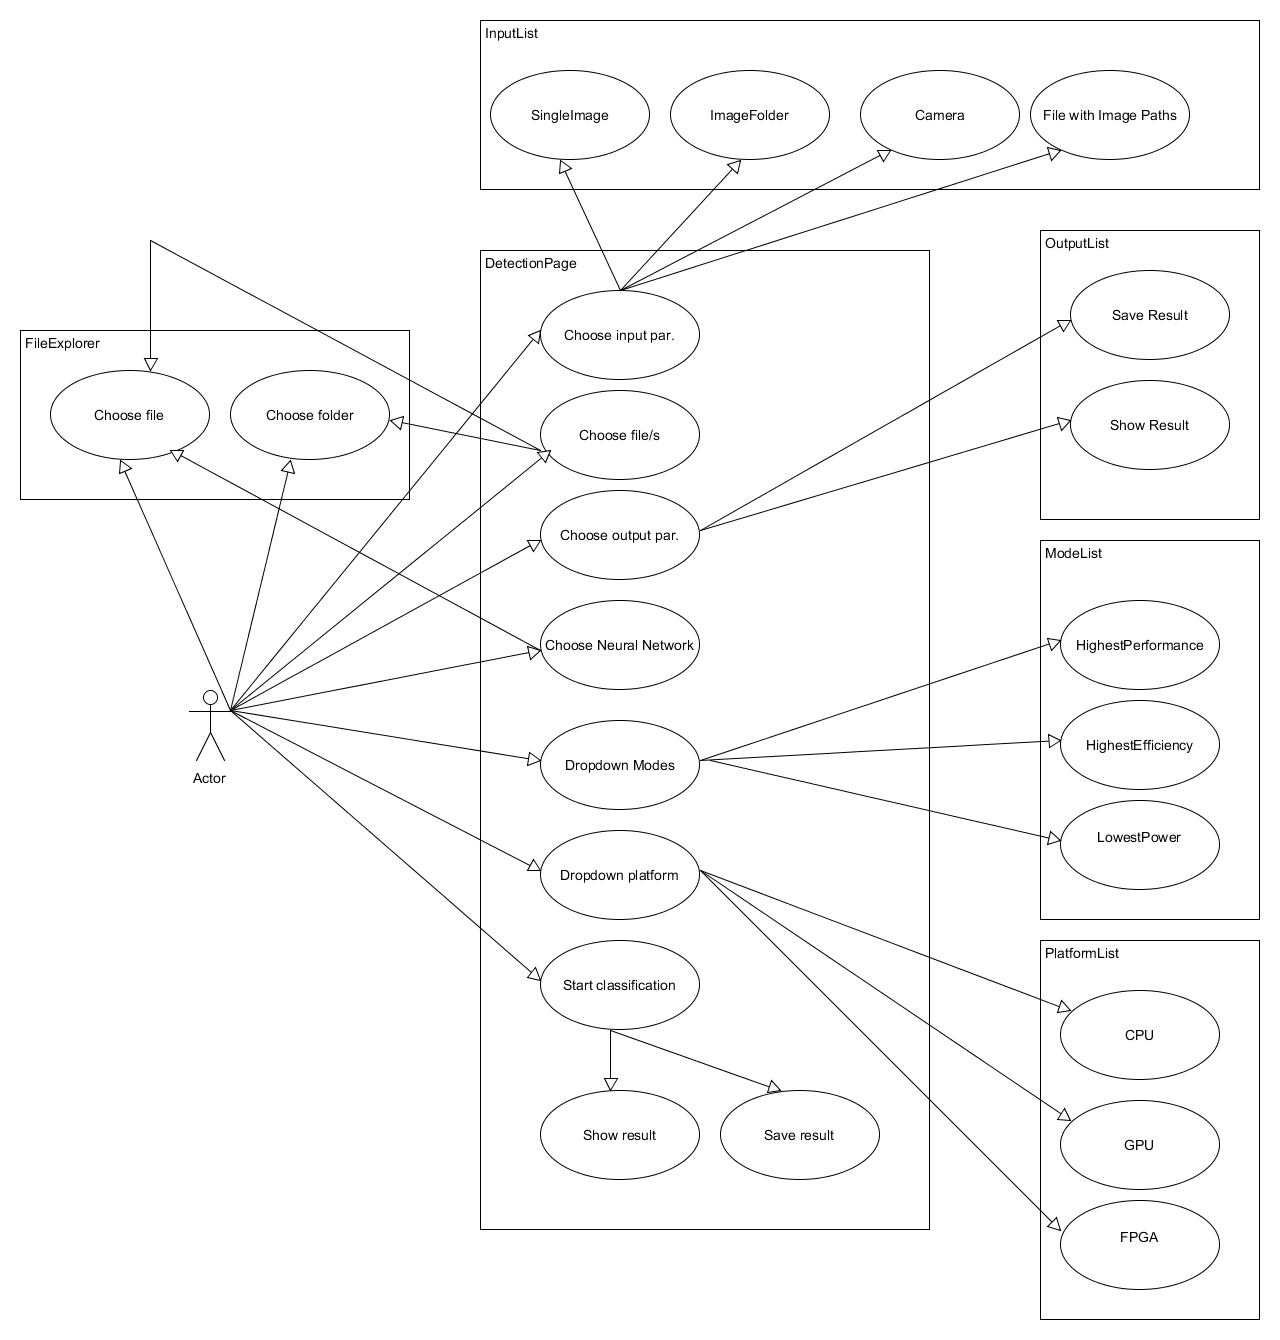
\includegraphics[width=\textwidth]{ClassificationUsecase}
\caption{Usecase of the \gls{image classification} page}
\end{figure}
\newpage
\subsubsection{Training page}
\begin{figure}[htb!]
\centering
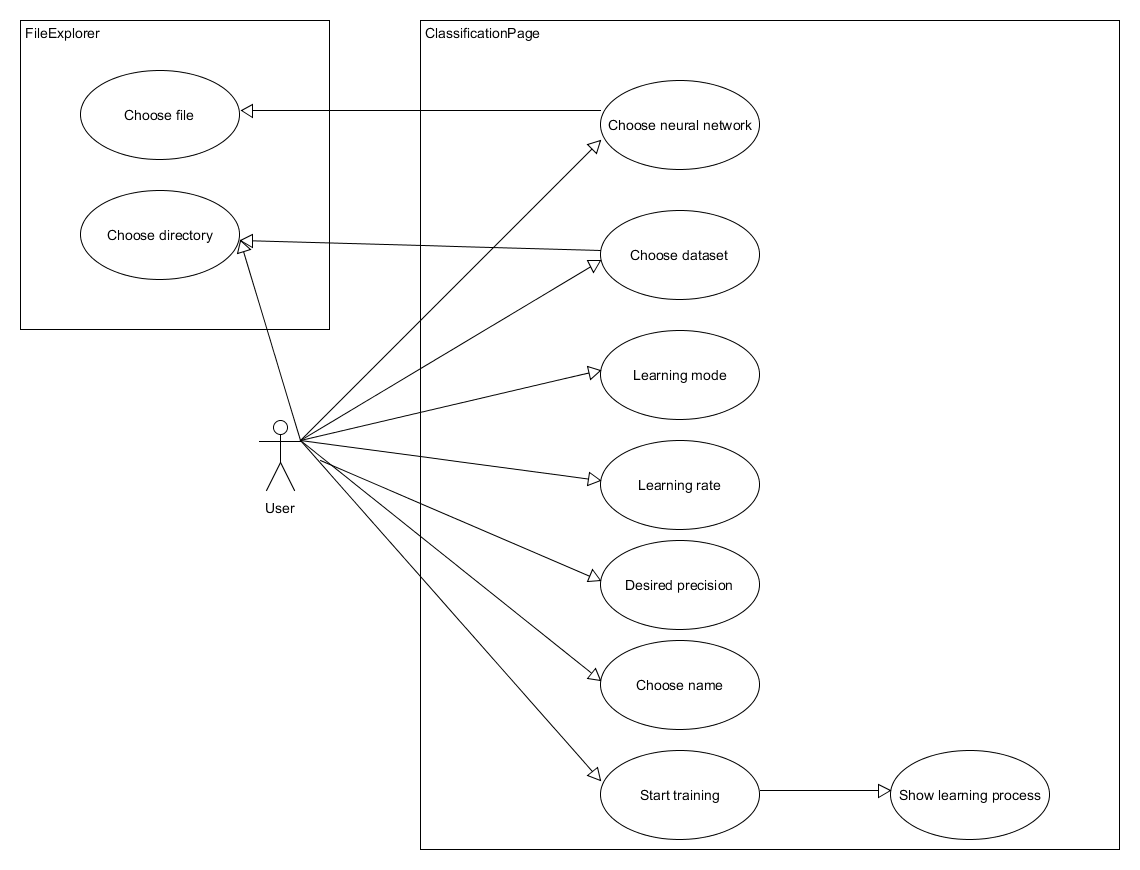
\includegraphics[width=\textwidth]{TrainUsecase}
\caption{Usecase of the trainingspage}
\end{figure}
\clearpage
\subsubsection{Image detection page}
\begin{figure}[htb!]
\centering
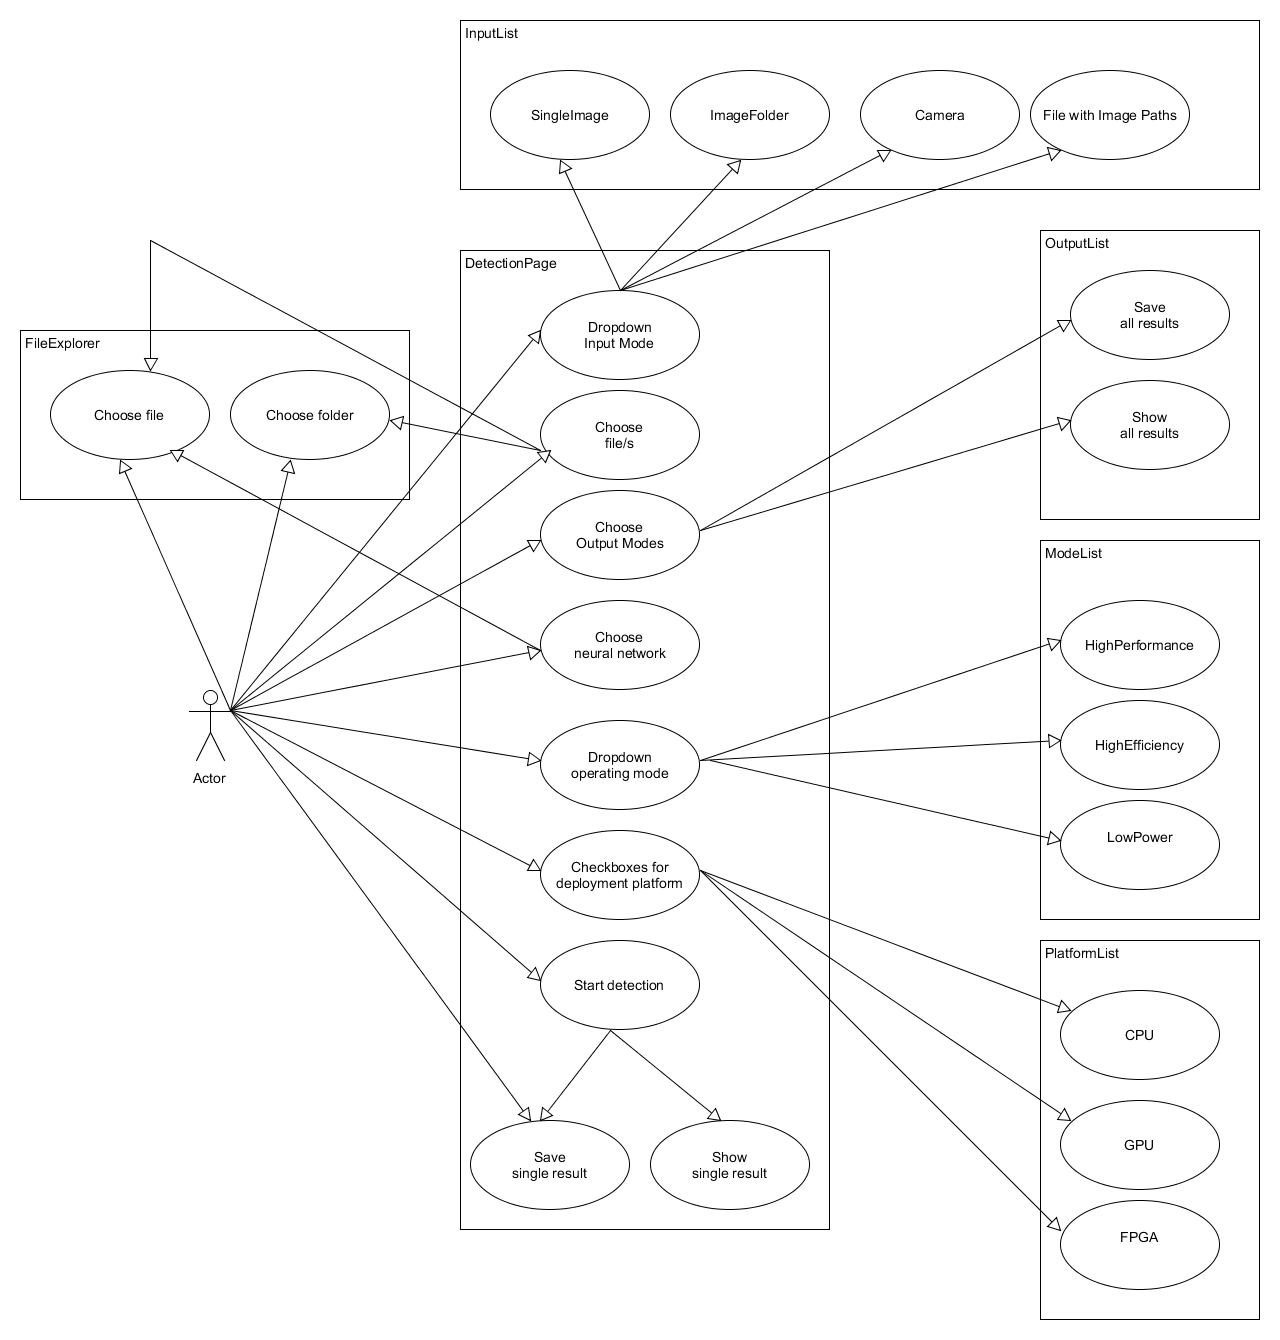
\includegraphics[width=\textwidth]{objectDetectionUsecase}
\caption{Usecase of the image detection page}
\end{figure}
\newpage
\subsubsection{Show topology page}
\begin{figure}[htb!]
\centering
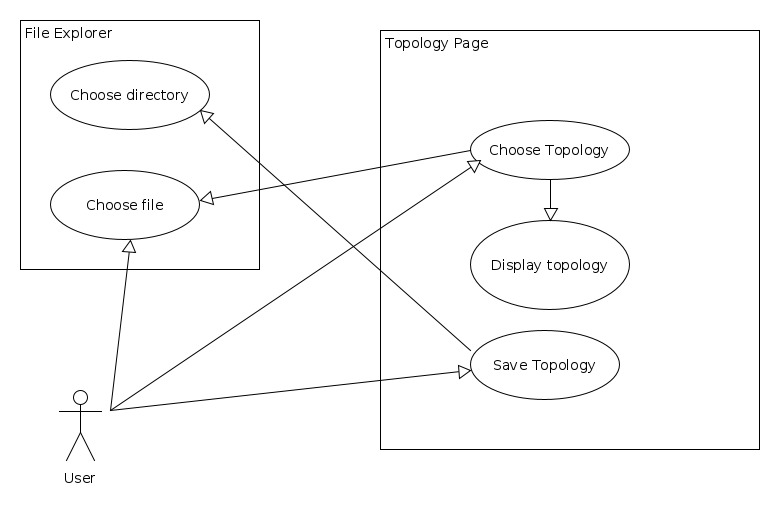
\includegraphics[width=\textwidth]{ShowTopoUsecase}
\caption{Usecase of the image classification page}
\end{figure}
\newpage

\subsection{GUI}
\begin{figure}[htb!]\centering
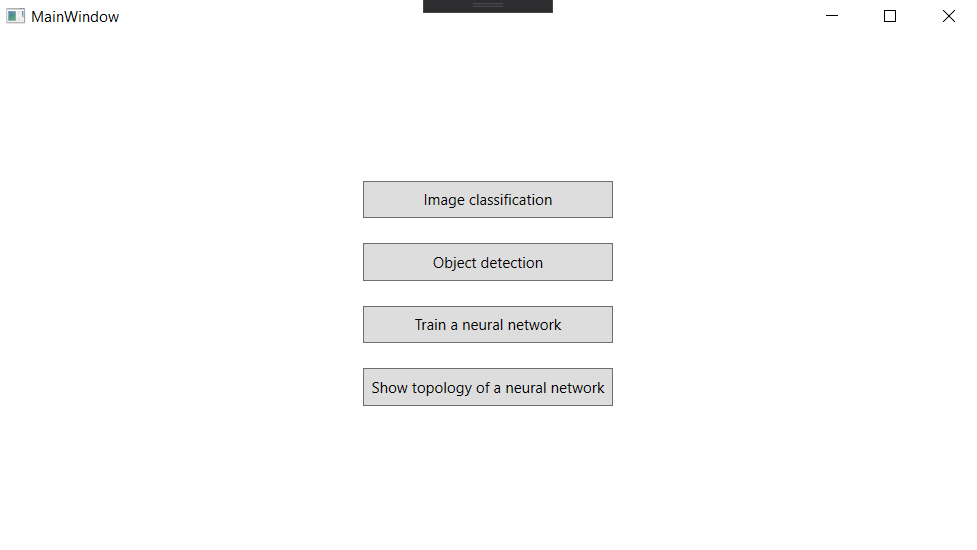
\includegraphics[width=\textwidth]{MainPageGUI}
\caption{Main page of our software}
\end{figure}
\begin{figure}[htb!]\centering
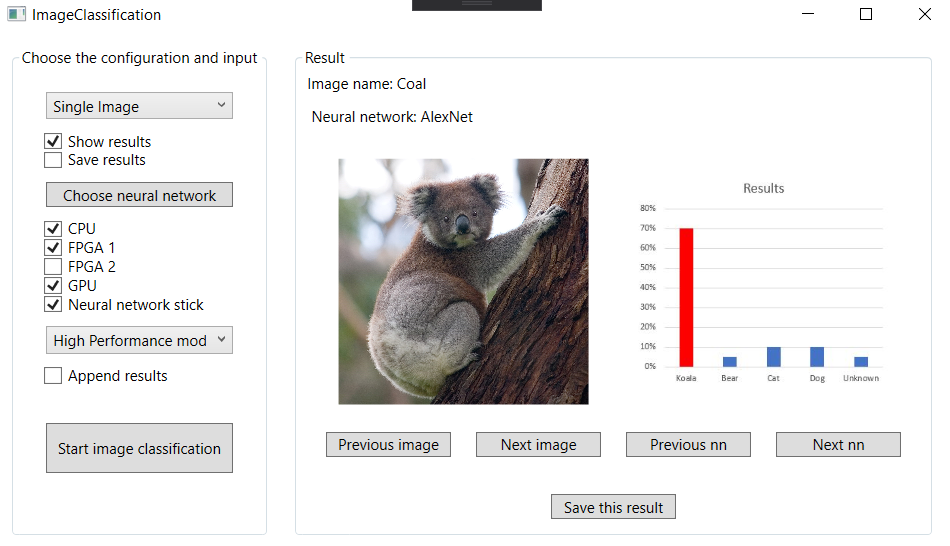
\includegraphics[width=\textwidth]{ImageClassificationGUI}
\caption{\gls{image classification} page of our software}
\end{figure}
\begin{figure}[htb!]\centering
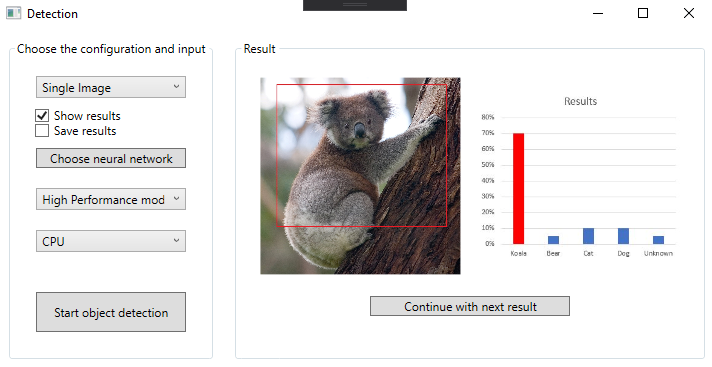
\includegraphics[width=\textwidth]{DetectionGUI}
\caption{Object detection page of our software}
\end{figure}
\begin{figure}[htb!]\centering
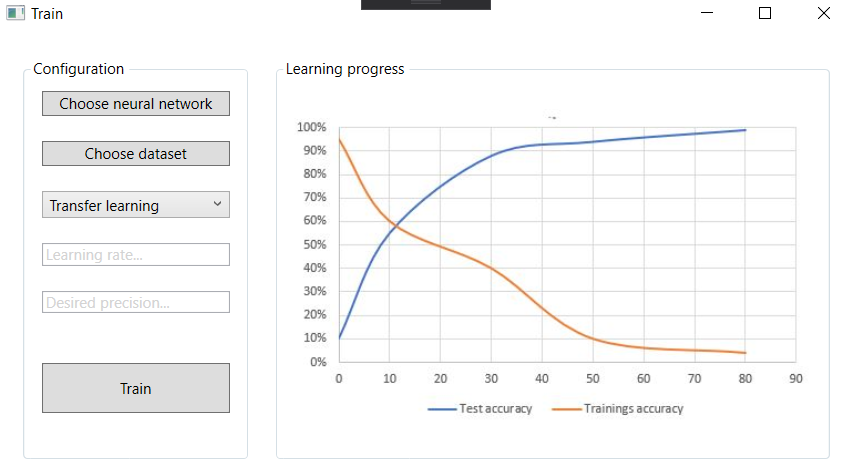
\includegraphics[width=\textwidth]{TrainGUI}
\caption{Training page of our software}
\end{figure}
\begin{figure}[htb!]
\centering
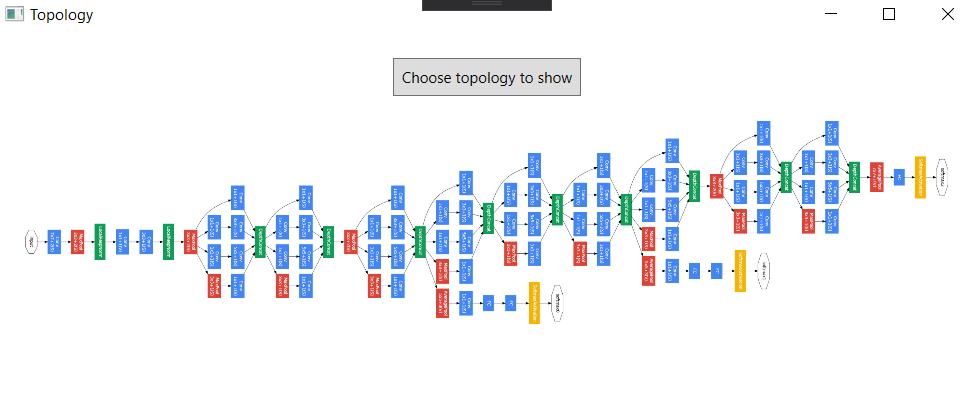
\includegraphics[width=\textwidth]{TopoGUI}
\caption{Page which shows the topology of a selected NN of our software}
\end{figure}
\clearpage

\section{Stage responsibilities}
\begin{tabular}{p{4cm}p{8cm}}
\textbf{Requirements:} & Paul Stangel\\
\textbf{Design:} & Johannes Häring\\
\textbf{Implementation:} & Manuel Drehwald\\
\textbf{Quality insurance:}& Stefani Guneshka\\
\textbf{Deployment:} & Dimitar Dimitrov
\end{tabular}

\section{Quality requirements}
\begin{tabular}{|p{3cm}|c|c|c|c|}
\hline
\textbf{Name} & \textbf{Very relevant} & \textbf{Relevant} & \textbf{Less relevant} & \textbf{Not relevant}\\
\hline
Failure tolerance & & & & \\
\hline
Security & & & & X \\
\hline
Usability & & X & & \\
\hline
Time requirement classification& X & & &\\
\hline
Time requirement detection& & X & &\\
\hline
\end{tabular}
\clearpage

\printnoidxglossaries
\end{document}

